\documentclass[12pt, a4paper]{article}
\usepackage[utf8]{inputenc}
\usepackage{indentfirst} %indentace prvního odstavce
\usepackage{url}
\usepackage{amsmath}
\usepackage{graphicx}
\usepackage[czech]{babel}
\usepackage{hyperref}

\graphicspath{ {pics/} }

\title{NMMB202 Zápočtový program - Šifrovací aplikace pro Android (Anigma)}
\author{Jan Oupický}
\date{2018}

\begin{document}
\maketitle

\section{Zadání}

Aplikace má umět šifrovat a i dešifrovat podle zadaných parametrů vstupní text a soubory. Použité šifry AES, 3DES apod.

\section{Uživatelský manuál}

Aplikace je dostupná ke stažení na Google Play pod jménem "Anigma". Odkaz ke stažení: \url{https://play.google.com/store/apps/details?id=xyz.honzaik.anigma}.

Po stažení stačí aplikaci zapnout. Aplikace si po spuštění vyžádá oprávnění ke čtení a zápisu souborů v telefonu, kvůli šifrování souborů viz \ref{fig:perm}. Pokud uživatel nedá aplikaci oprávnění, tak se aplikace vypne.

Jestliže aplikace dostala potřebné oprávnění tak se zobrází hlavní a jediné okno aplikace viz \ref{fig:main}. Úplně nahoře jsou 2 tlačítka označení "TEXT MODE" a "FILE MODE". Pomocí těchto tlačítek si může uživatel vybírat zda-li chce šifrovat text \ref{fig:main} nebo soubory \ref{fig:file}. Pod těmito tlačítky je další možnost výběru a to z dostupných šifer \ref{fig:ciphers}. V aktuální verzi (1.0) jsou v aplikaci pouze dostupné šifry AES-128, AES-256 a 3DES plánuje se podpora šifer Serpent a Twofish (finalisté AES).

Nyní si probereme samostatně "TEXT MODE" a "FILE MODE".

\subsection{Textový mód}
Následující dvojicí tlačítek po výběru šifry jsou tlačítka s označením "ENCRYPTION" a "DECRYPTION". Pomocí nich si uživatel může vybrat, zda chce text šifrovat nebo dešifrovat. 

Pokud si vybere šifrování. Tak se mu zobrazí toto rozhraní \ref{fig:main}. Do políčka "Plaintext" stačí vyplnit požadovaný text, jenž chce uživatel zašifrovat. Dále do políčka "Password (key)" uživatel vyplní heslo, pomocí kterého se odvodí klíč k zašifrování textu. Posledním políčkem je políčko pro inicializační vektor (IV), uživatel si může vyplnit vlastní inicializační vektor, ale musí mít správou délku pro vybranou šifru a být zakódován v Base64. Toto se nedoporučuje, a proto je hned vedle tlačítko "GENERATE RANDOM", které vygeneruje správně náhodný inicializační vektor.

Dále má uživatel možnost si inicializační vektor zkopírovat do schránky, ale to obvykle není potřeba, jelikož nemusí být tajný narozdíl od hesla a automaticky se přidává do šifrového textu.

Nakonec stačí stisknout tlačítko "ENCRYPT STRING", která zahájí šifrování. Zobrazí se načítací kolečko, které informuje, že šifrování právě probíhá. Obvykle šifrování ale proběhne tak rychle, že ho uživatel nespatří. Pokud vše proběhlo v pořádku, tak by se měl výsledek zobrazit v okénku pod tlačítkem "COPY RESULT TO CLIPBOARD", který zašifrovaný text zkopíruje do schránky \ref{fig:text_enc_success}. Jesliže nastala chyba, bude na to uživatel upozorněn viz \ref{fig:text_enc_error}.

Dešifrování probíhá obdobně. Nyní již není potřeba vyplňovat IV, jelikož je součástí zašifrovaného textu \ref{fig:text_dec_success}.

\subsection{Souborový mód}
V tomto módu si uživatel podobně může vybrat mezi šifrováním a dešifrováním jako v textovém módu, ale předtím má na výběr z daných souborů \ref{fig:file}. Aplikace uživateli napoví, kde se nachazí složka aplikace, kde se se soubory pracuje. V tomto případě to je \texttt{/storage/emulated/0/Anigma}.

Následně uživatel vidí seznam dostupných souborů v této složce a může si z nich vybírat. Vybraný soubor je označen sytě nažloutlou barvou \ref{fig:file_chosen}.

Nyní již stačí postupovat obdobně jako v textovém módu. Po zahájení šifrování a dešifrování se objeví "progress bar", která označuje kolik je již zašifrováno dat ze souboru \ref{fig:progress}. Jestliže zašifrování proběhlo úspěšně, tak se v dolním okně zobrazí hláška "Succesffully encrypted file" a v seznamu souborů, by se měl objevit soubor s sufixem "encrypted.0" (nebo jiné číslo v závilosti na duplicitě) \ref{fig:file_enc_success}.

Dešifrování probíhá obdobně. Po úspěšném dešifrování se vytvoří nový soubor s dalším sufixem "decrypted.0" \ref{fig:file_dec_success}.

\section{Závěr}
Aplikace je plně funkční, i když v aktuální verzi nepodporuje mnoho šifer. Naštěstí přidání podpory dalších šifer je snadné. Dalším vylepšením této aplikace by mohlo být integrování samostatného prohlížeče souboru, aby nebylo potřeba pořád kopírovat soubory do složky aplikace. Zdrojový kód je také k dispozici na \url{https://github.com/Honzaik/Anigma}.

\begin{figure}[h]
\caption{Požadavek na získání oprávnění.}
\centering
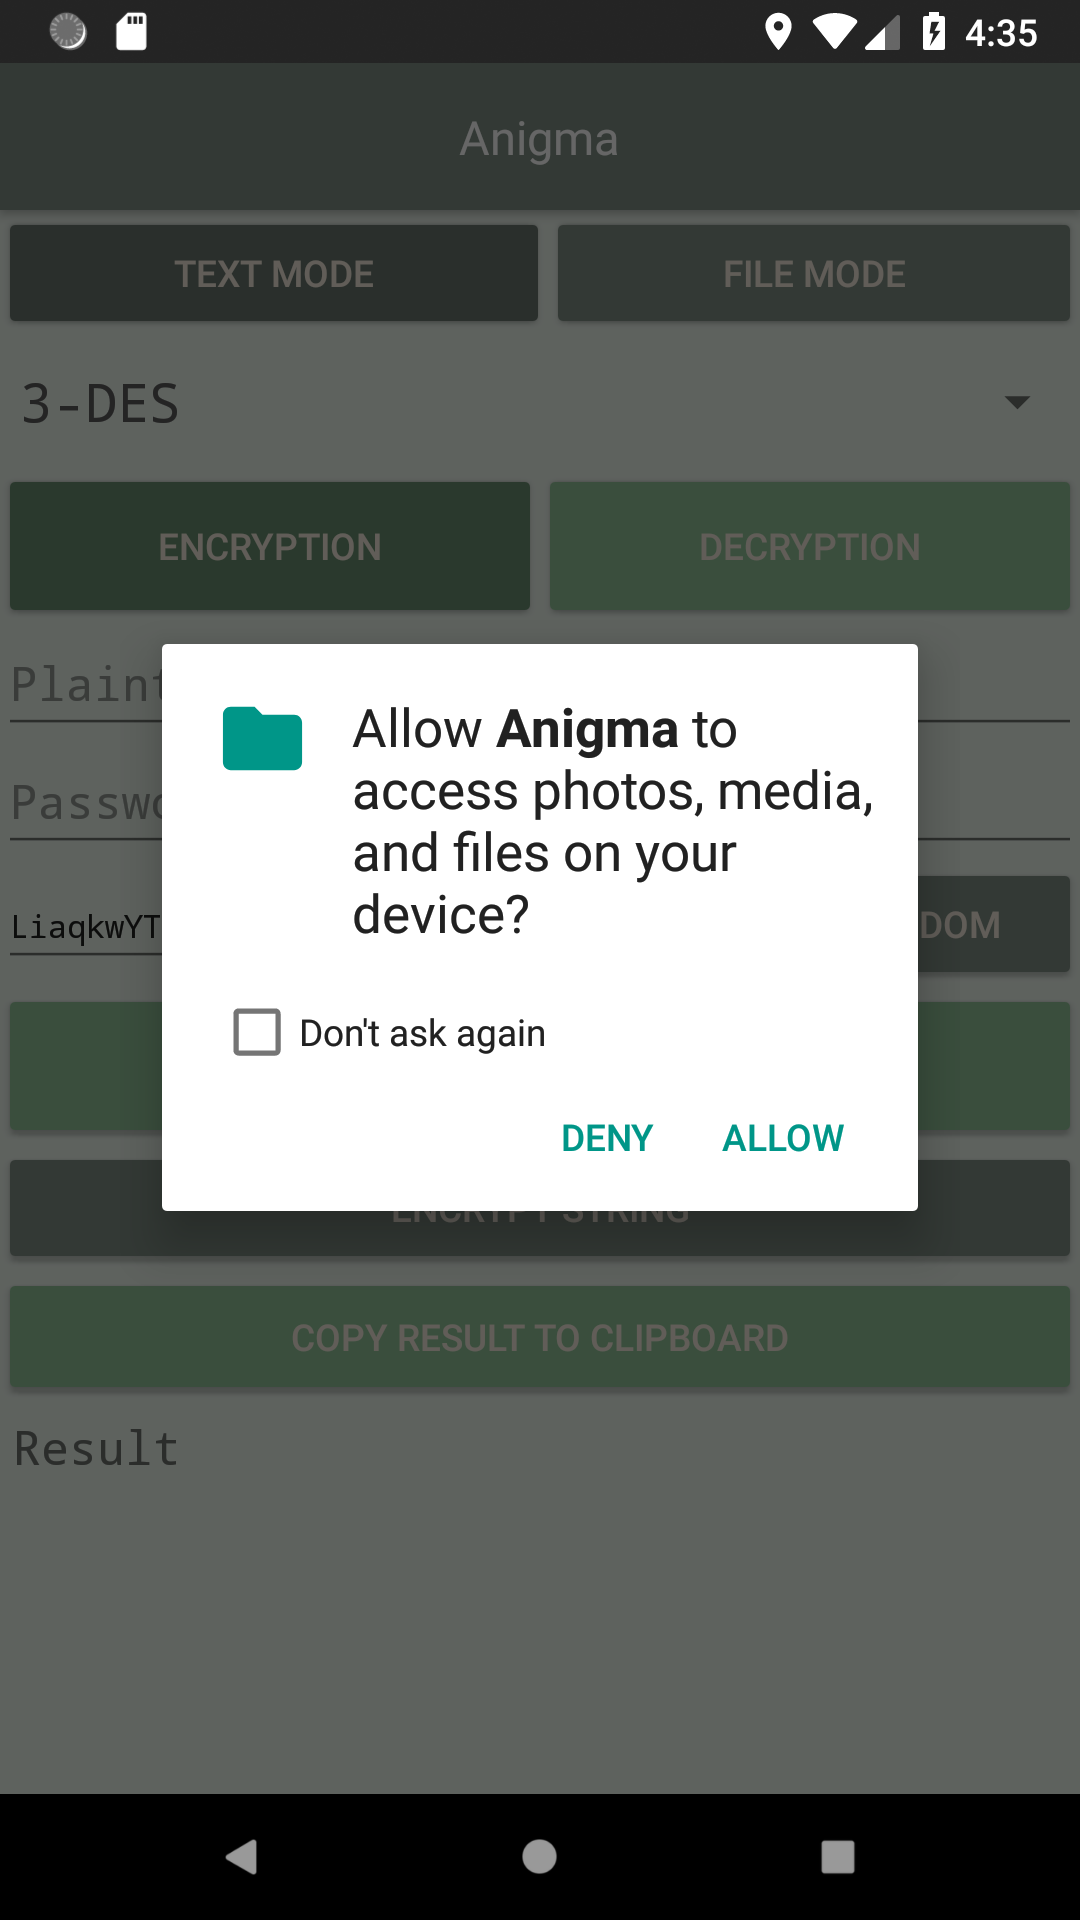
\includegraphics[height=0.4\textheight]{opravneni}
\label{fig:perm}
\end{figure}

\begin{figure}[h]
\caption{Hlavní okno - text mode (šifrování).}
\centering
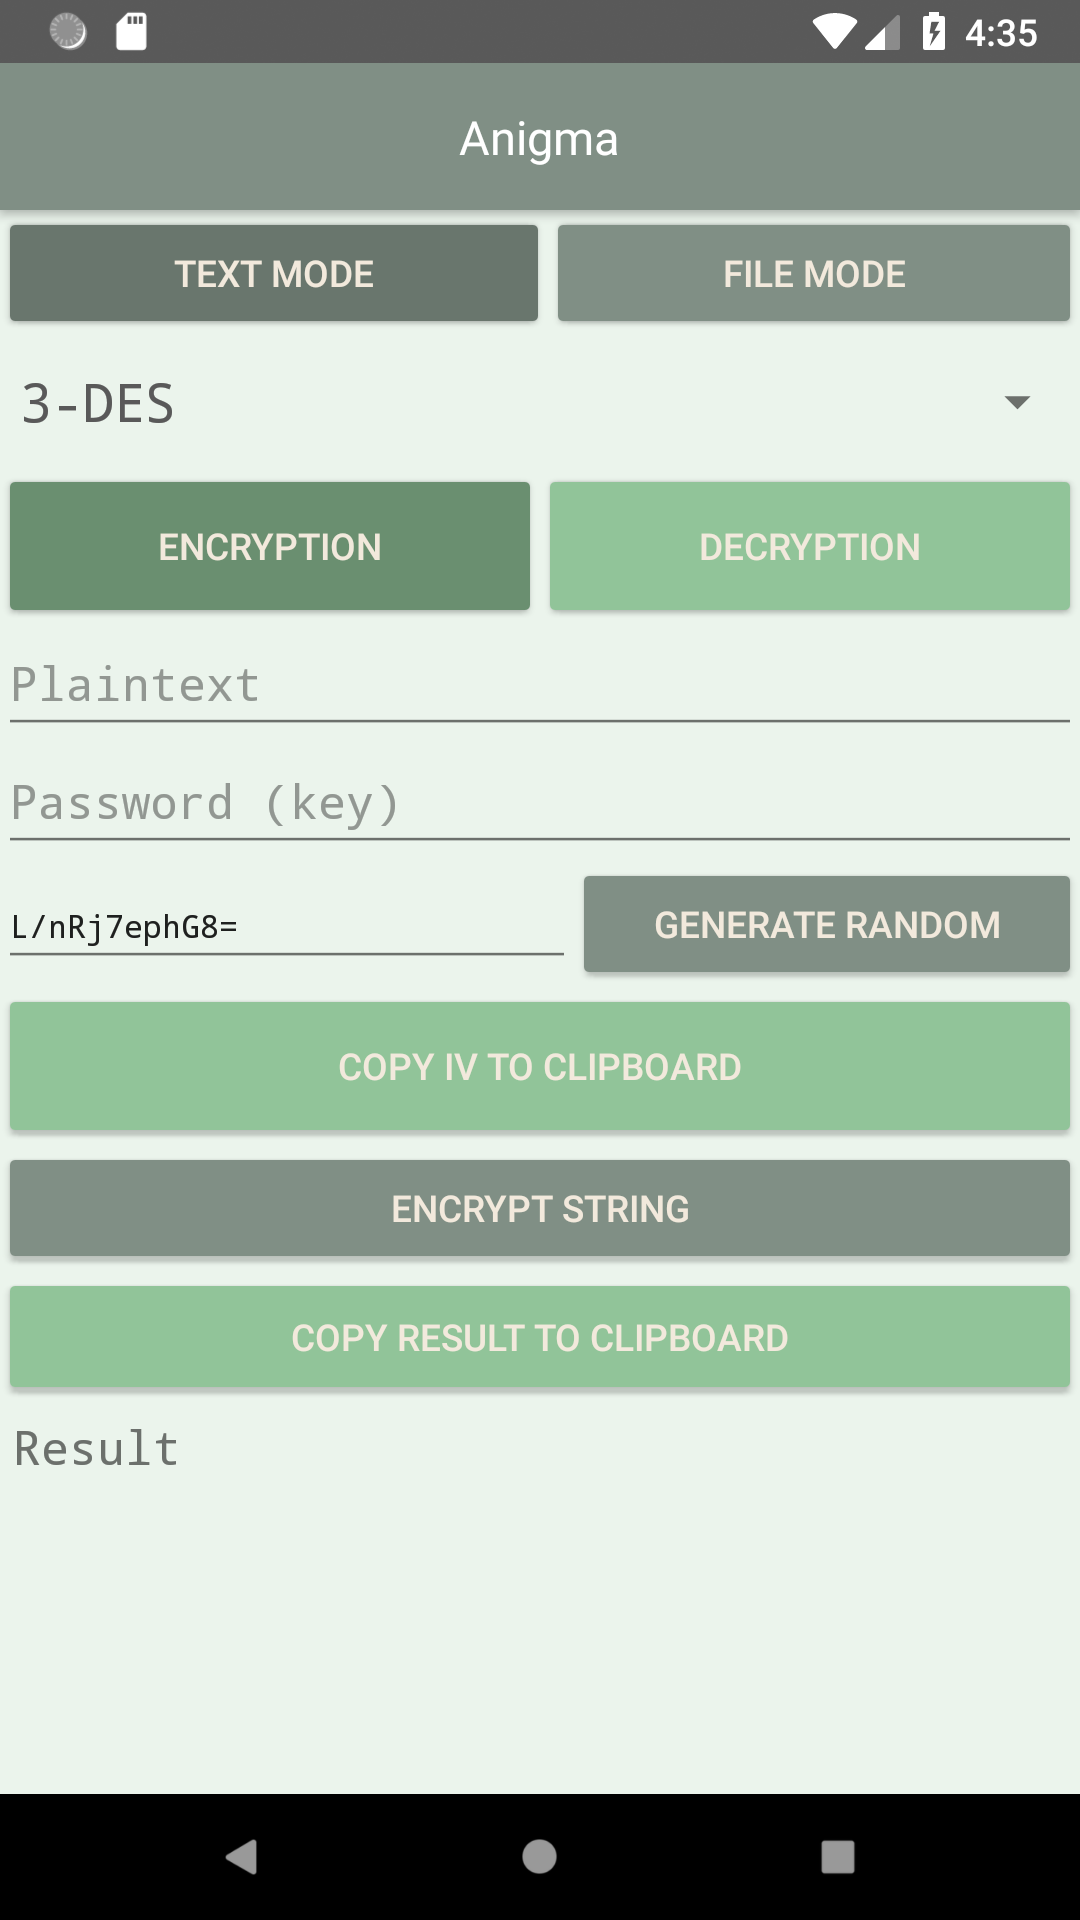
\includegraphics[height=0.4\textheight]{main}
\label{fig:main}
\end{figure}

\begin{figure}[h]
\caption{Hlavní okno - file mode.}
\centering
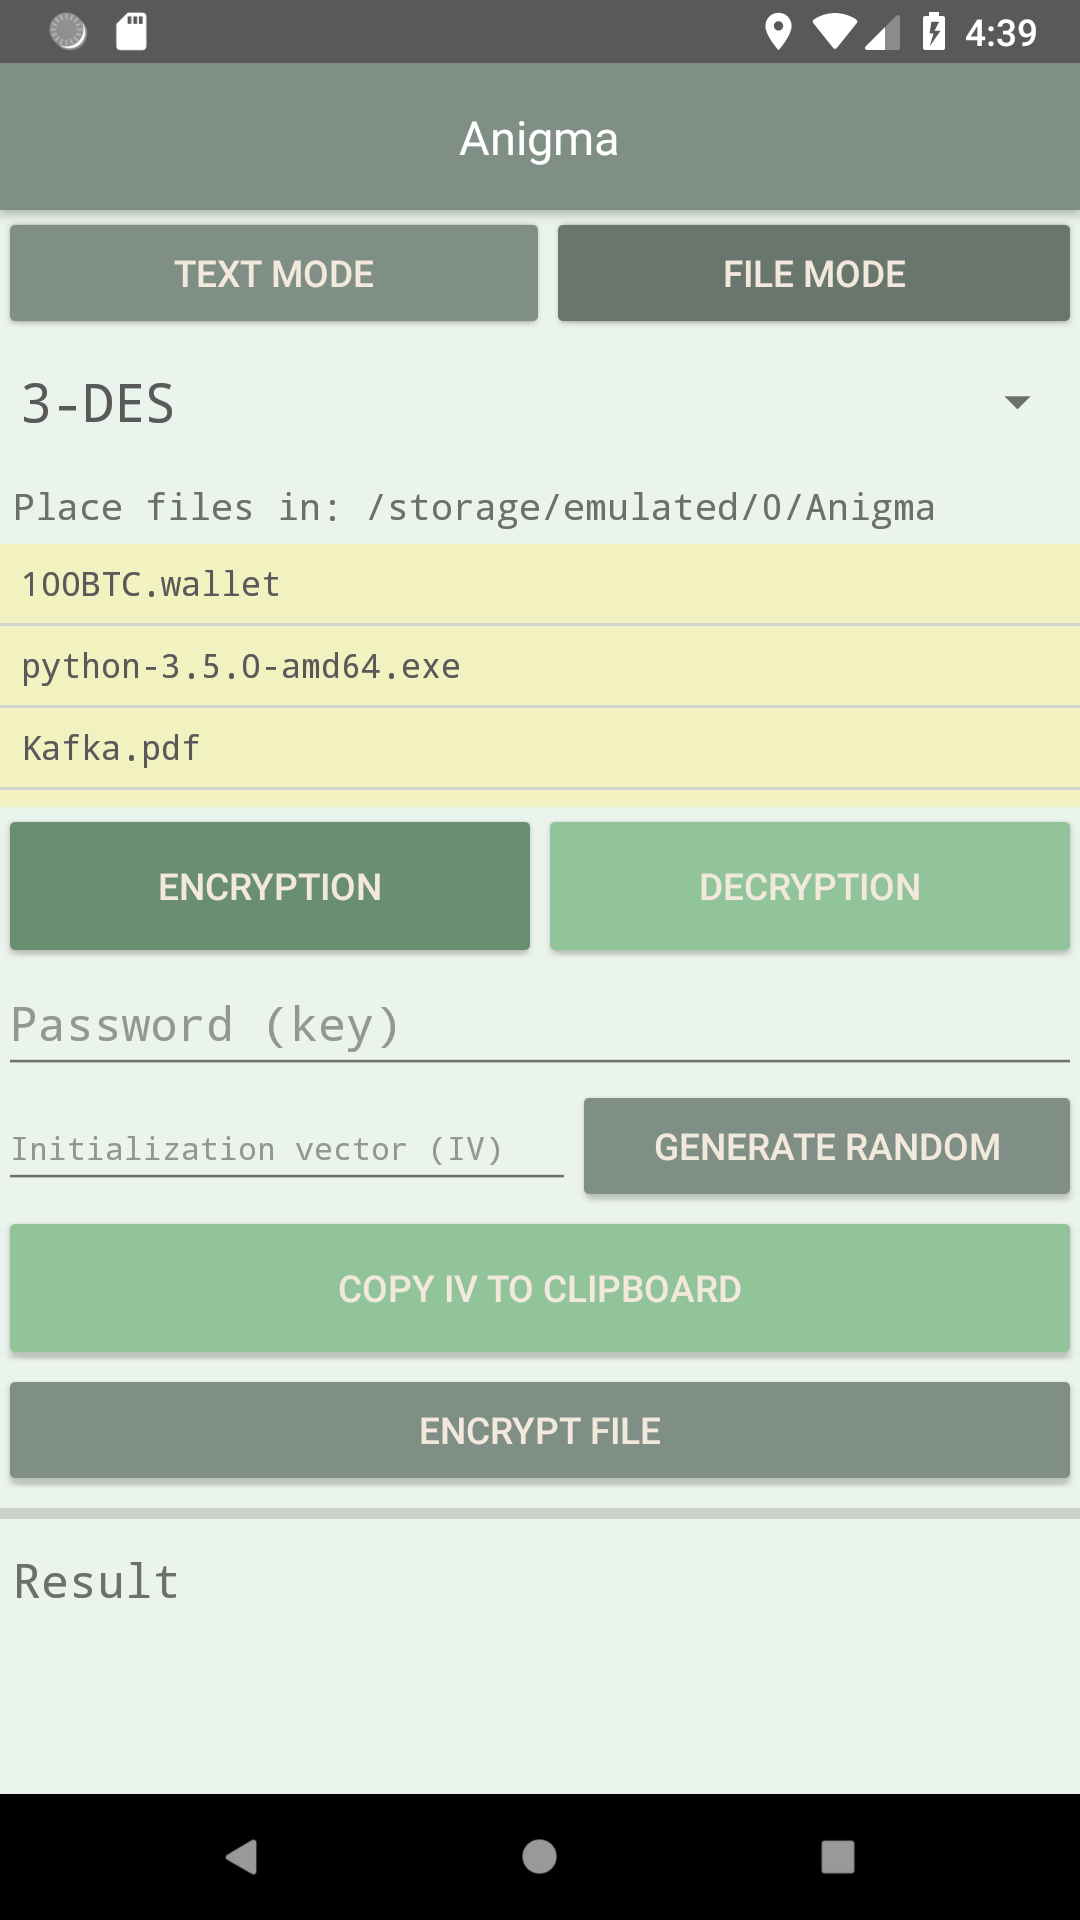
\includegraphics[height=0.4\textheight]{file}
\label{fig:file}
\end{figure}

\begin{figure}[h]
\caption{Seznam šifer.}
\centering
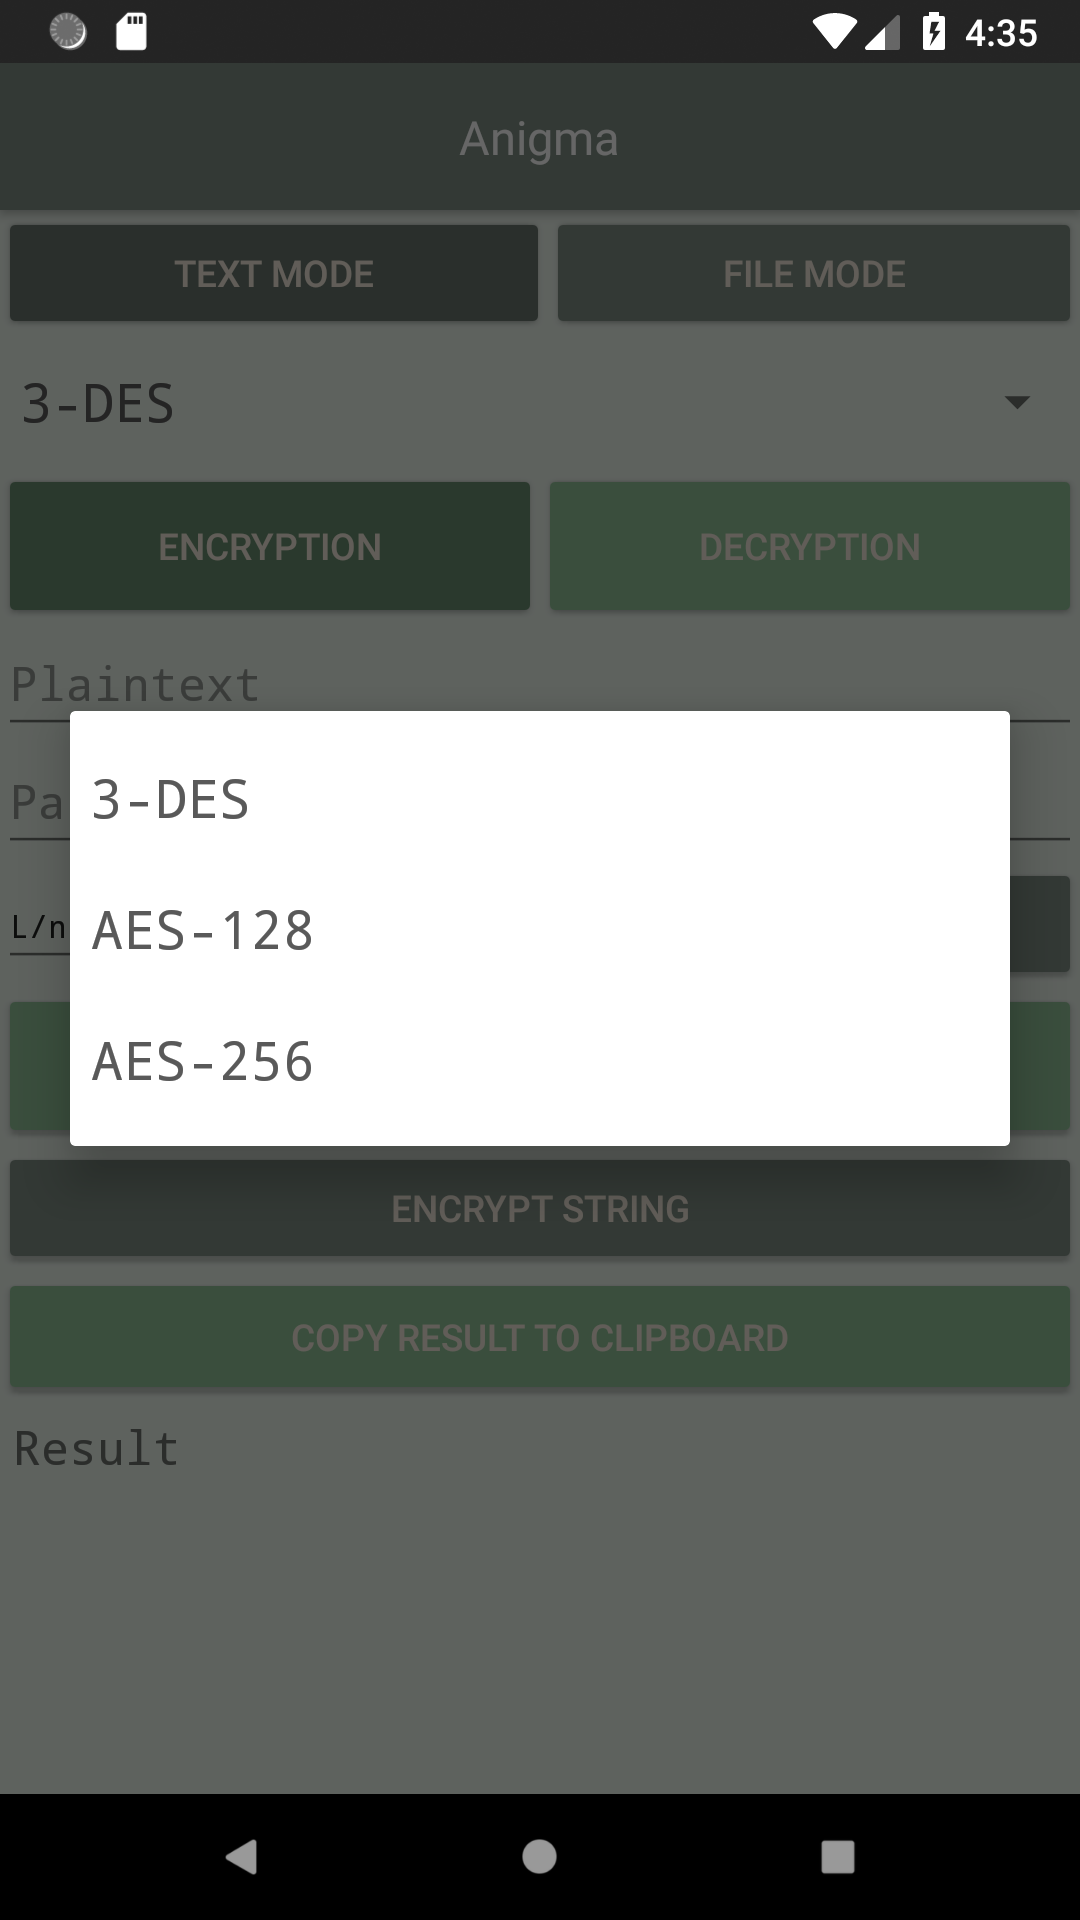
\includegraphics[height=0.4\textheight]{ciphers}
\label{fig:ciphers}
\end{figure}

\begin{figure}[h]
\caption{Textový mód - dešifrování.}
\centering
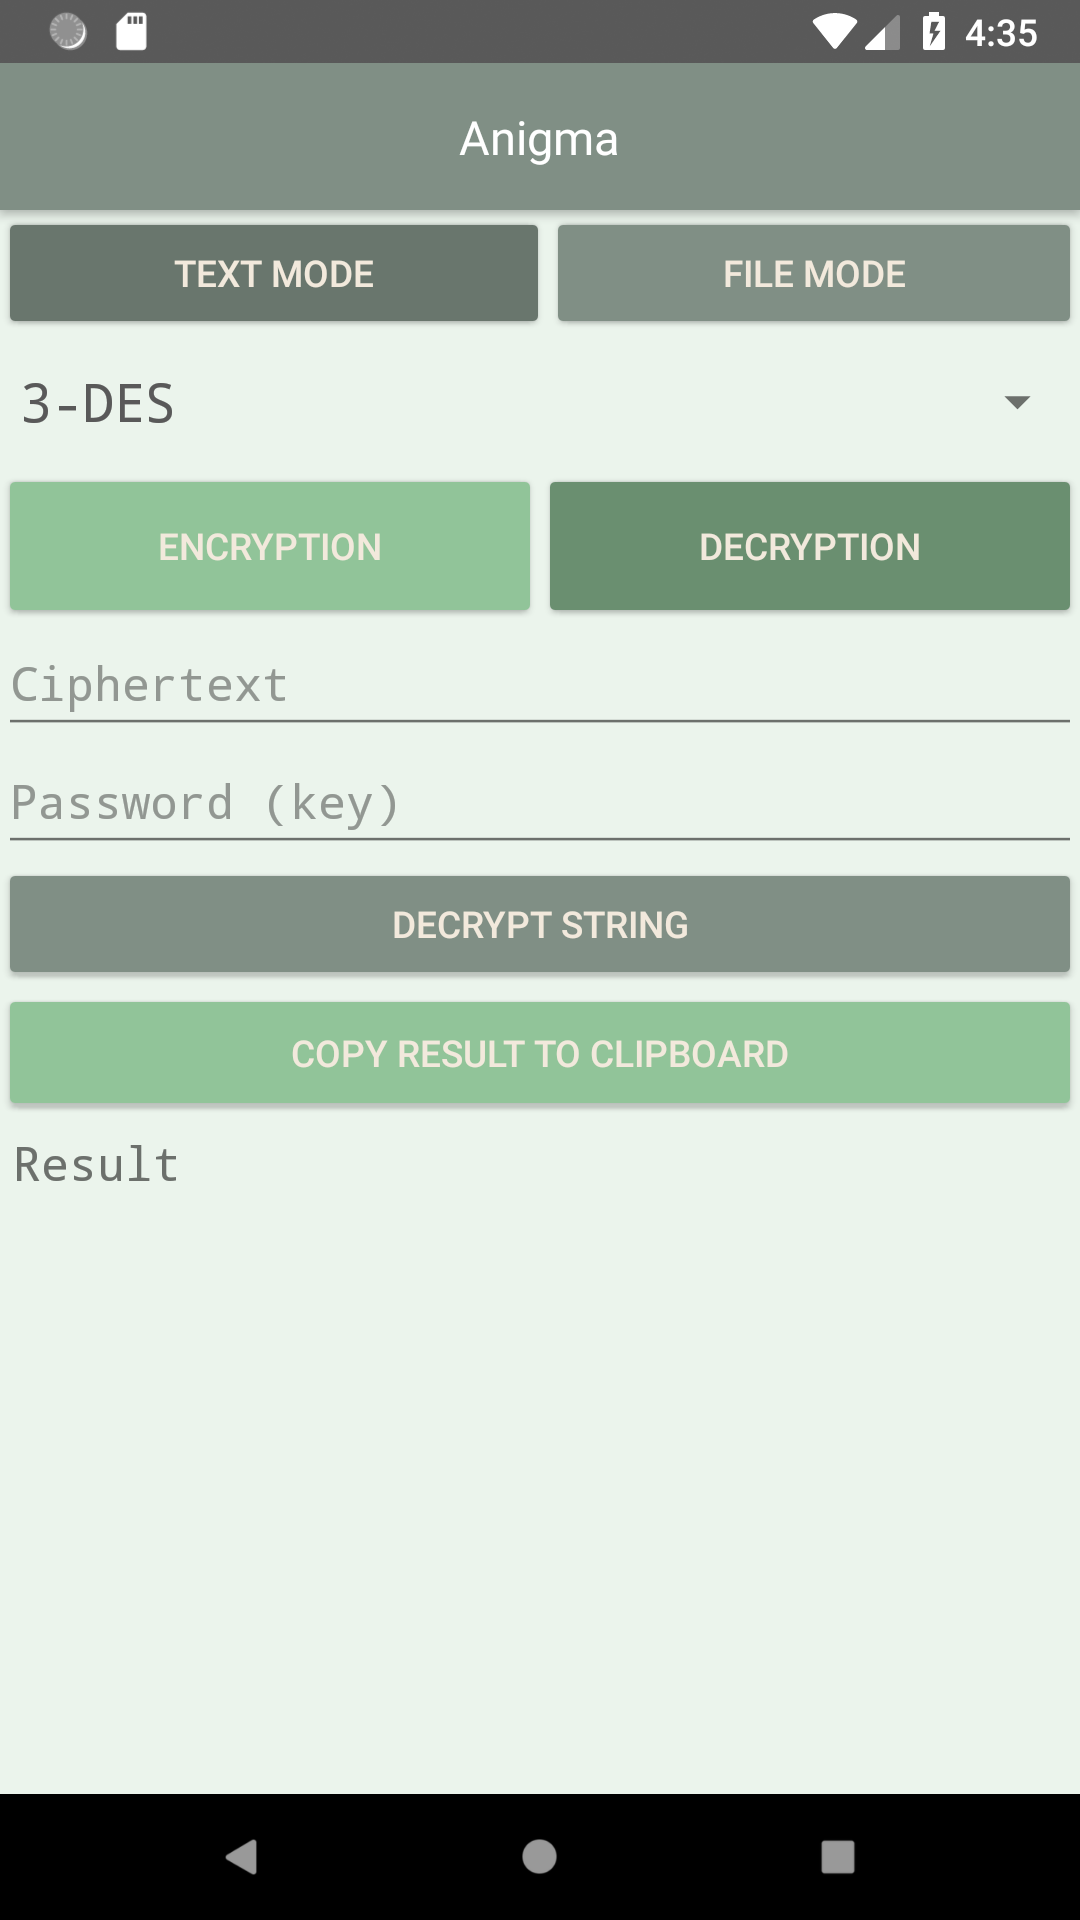
\includegraphics[height=0.4\textheight]{text_dec}
\label{fig:text_dec}
\end{figure}

\begin{figure}[h]
\caption{Úspěšné zašifrování textu.}
\centering
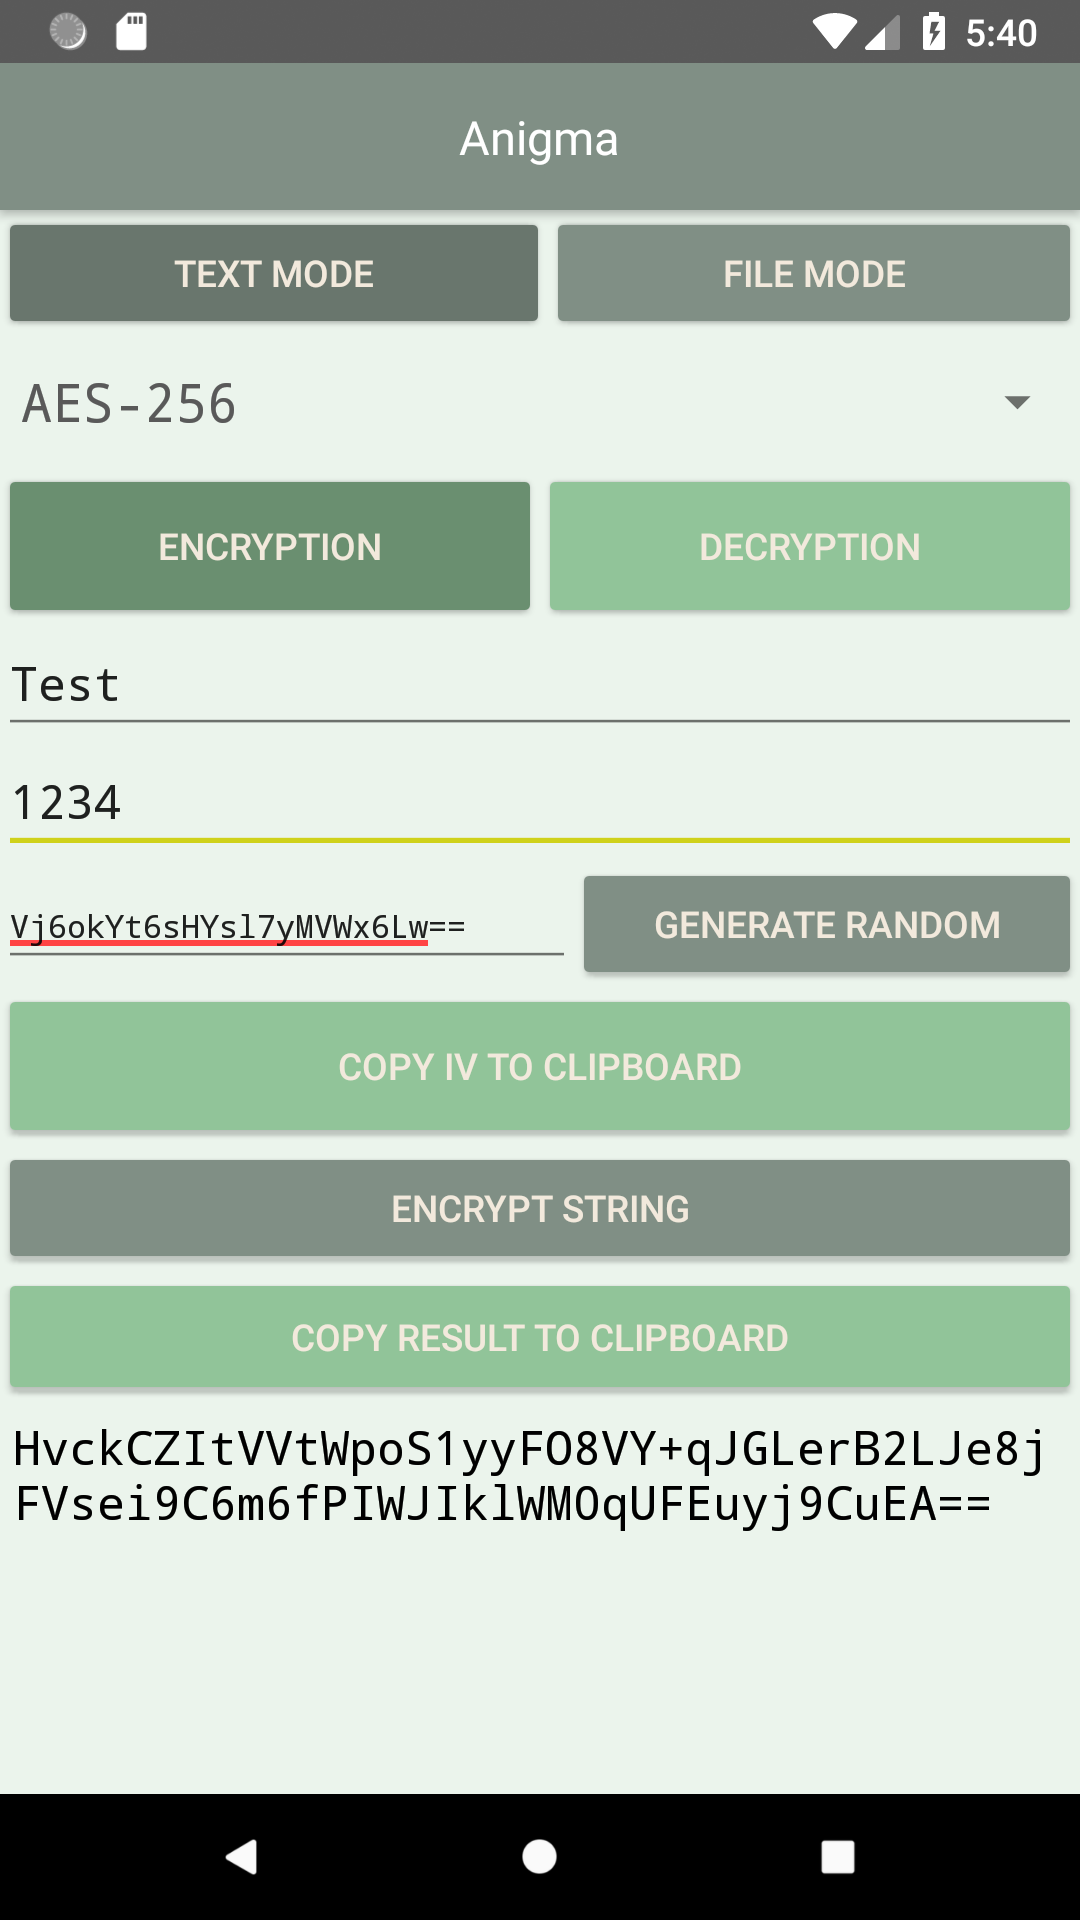
\includegraphics[height=0.4\textheight]{text_enc_success}
\label{fig:text_enc_success}
\end{figure}

\begin{figure}[h]
\caption{Neúspěšné zašifrování textu.}
\centering
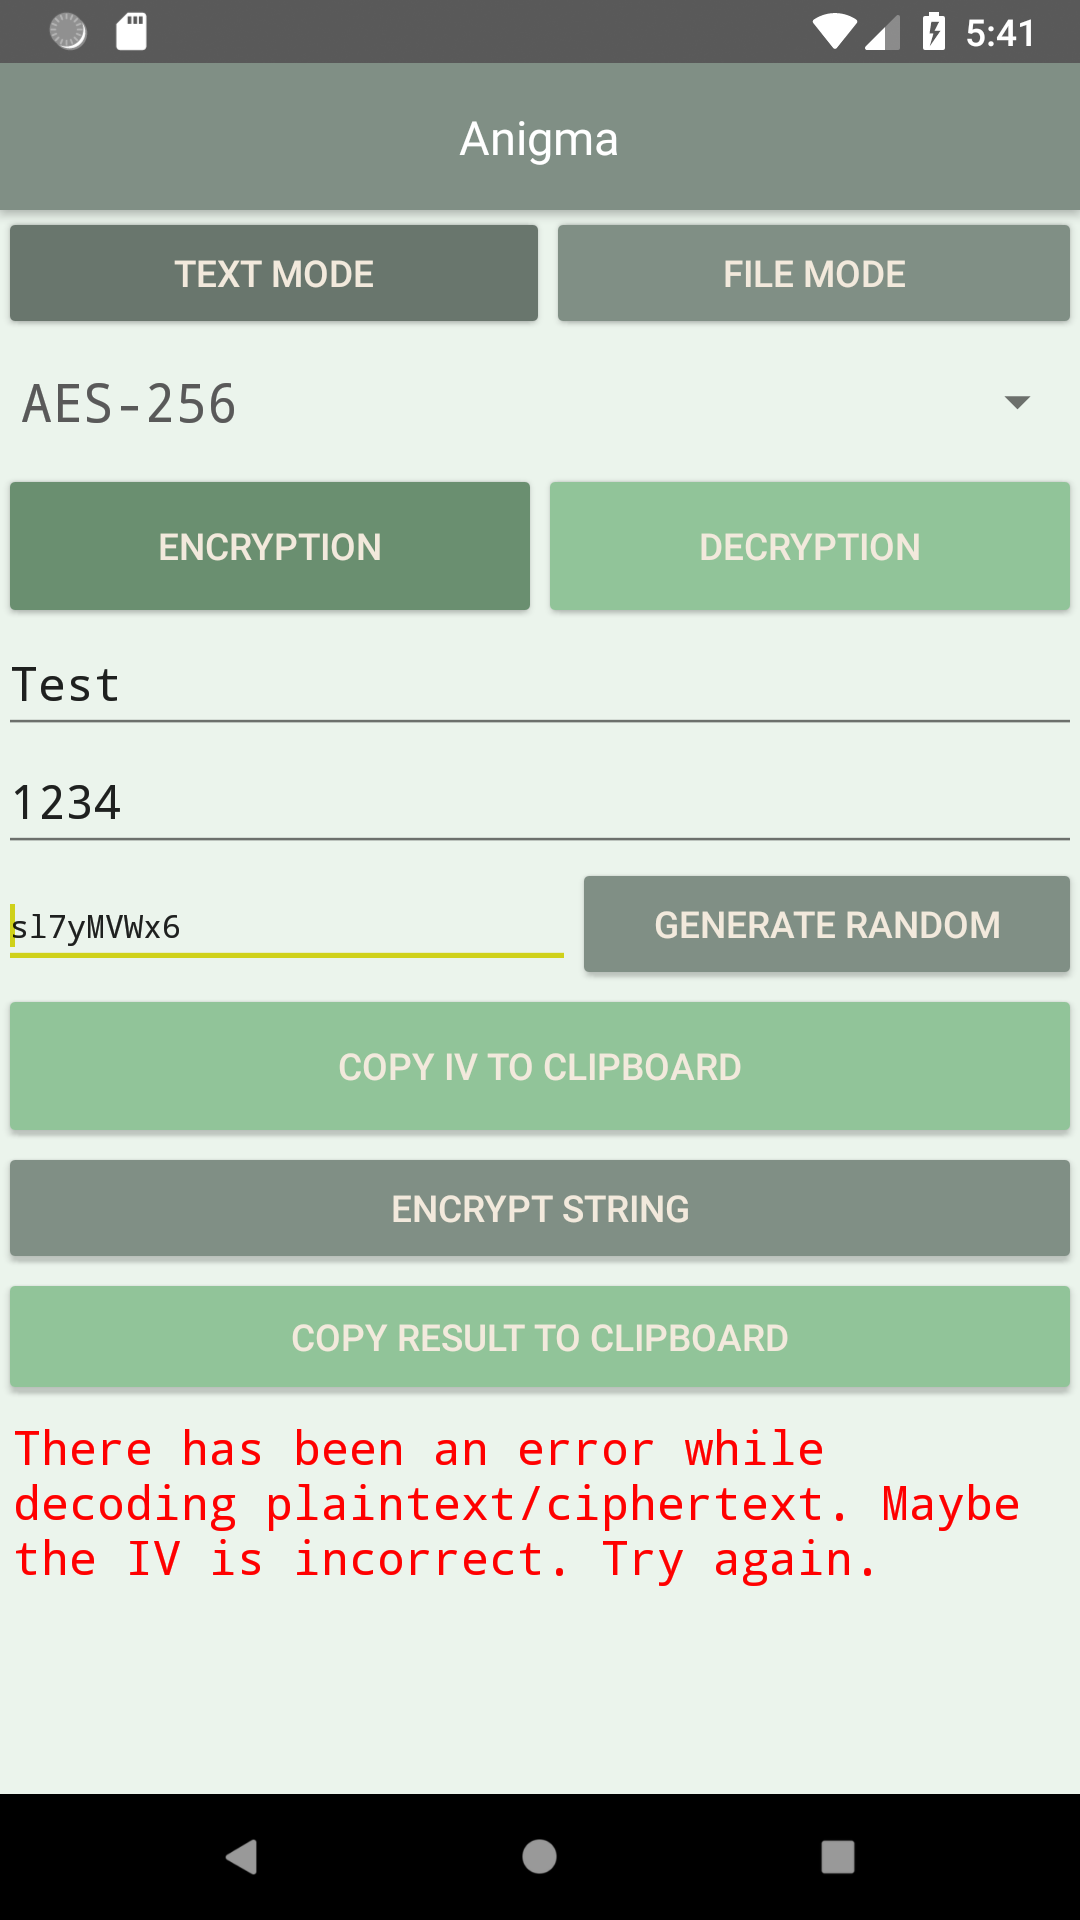
\includegraphics[height=0.4\textheight]{text_enc_error}
\label{fig:text_enc_error}
\end{figure}

\begin{figure}[h]
\caption{Úspěšné dešifrování textu.}
\centering
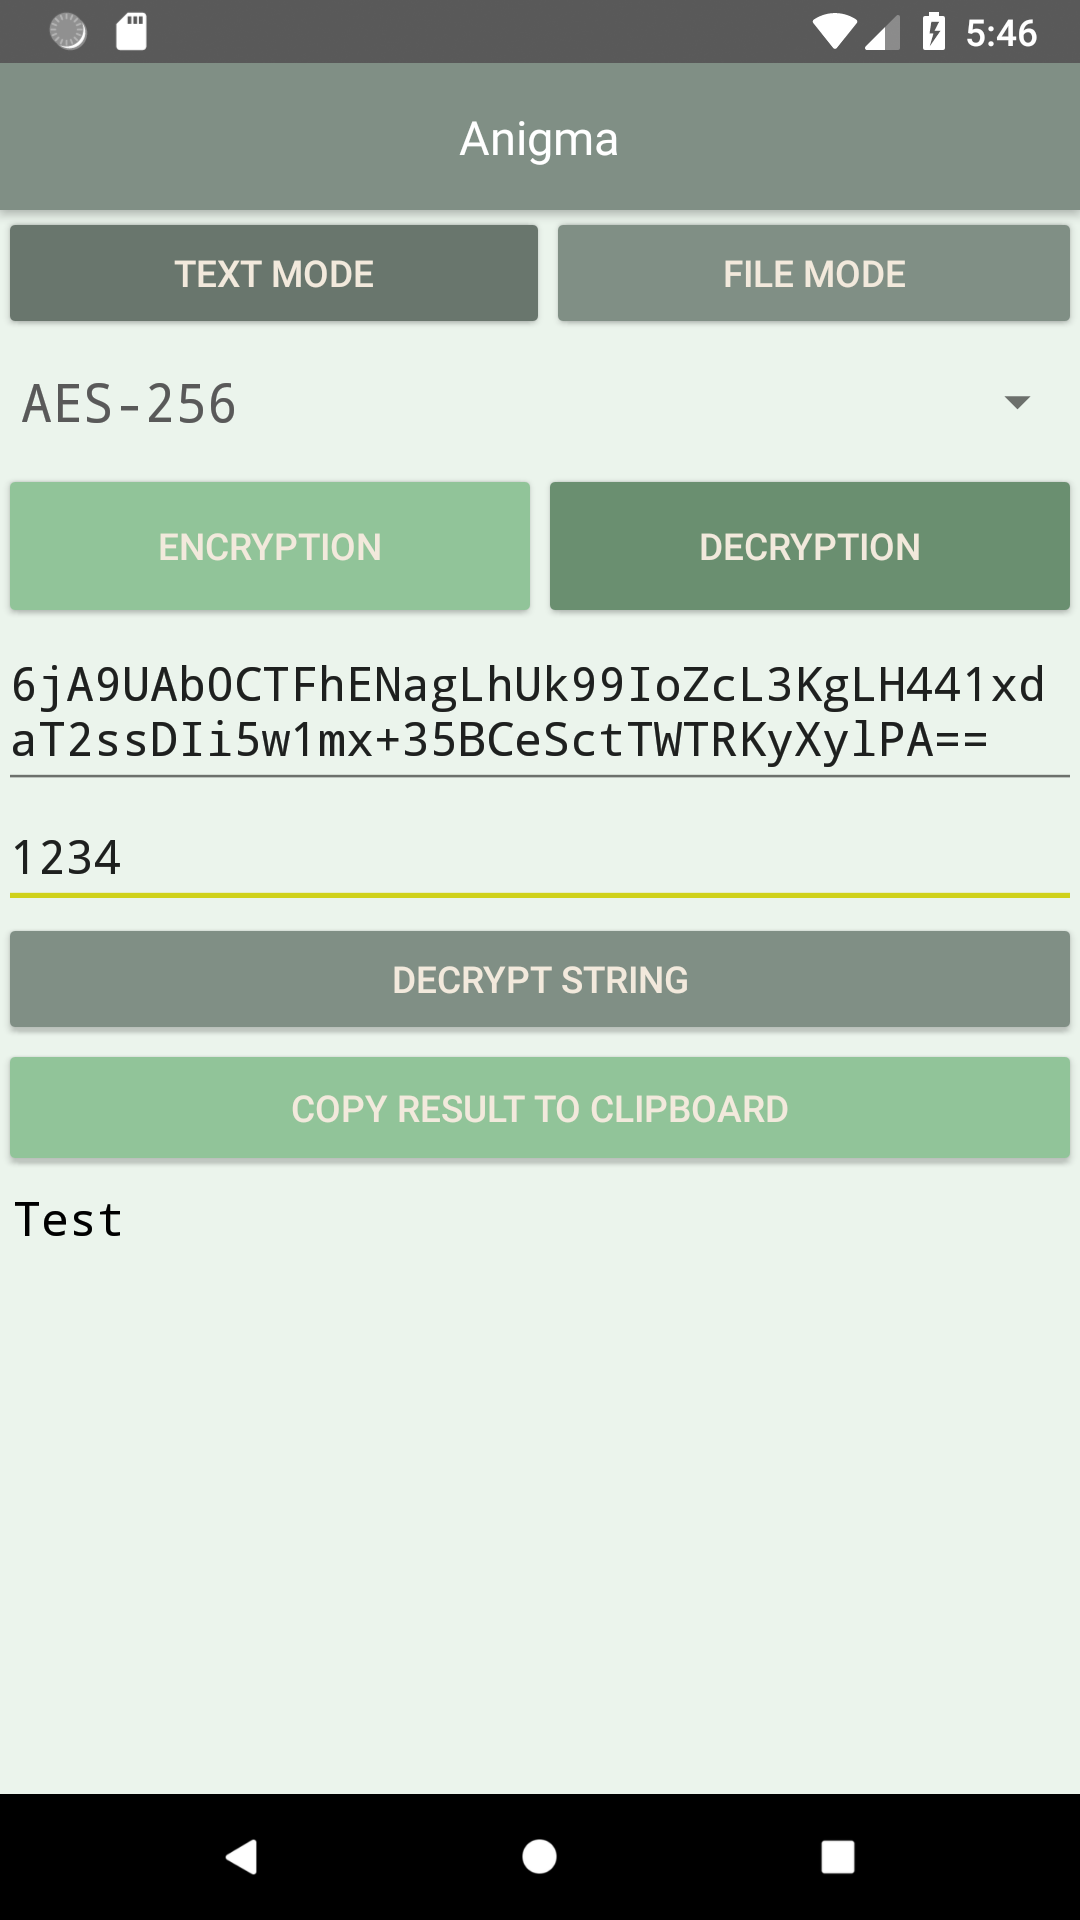
\includegraphics[height=0.4\textheight]{text_dec_success}
\label{fig:text_dec_success}
\end{figure}

\begin{figure}[h]
\caption{Vybrání souboru.}
\centering
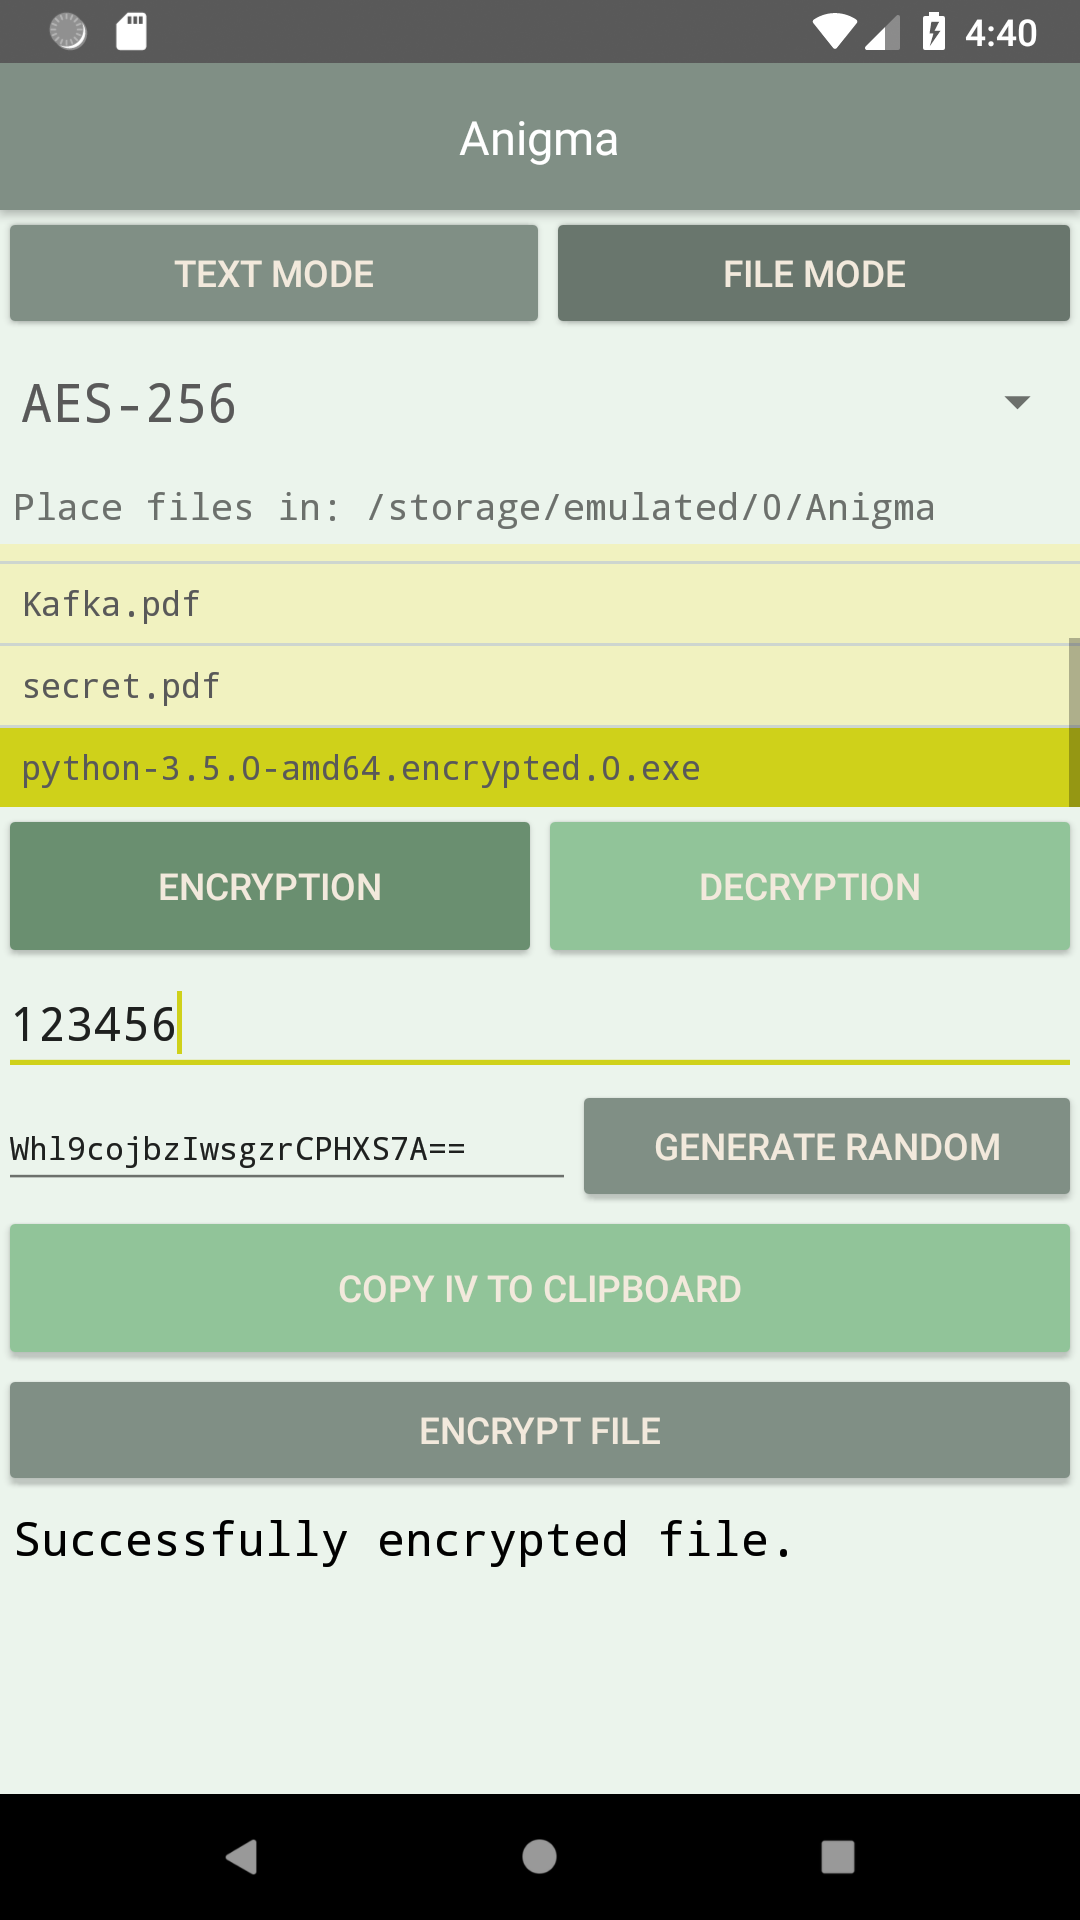
\includegraphics[height=0.4\textheight]{file_chosen}
\label{fig:file_chosen}
\end{figure}

\begin{figure}[h]
\caption{Progress bar.}
\centering
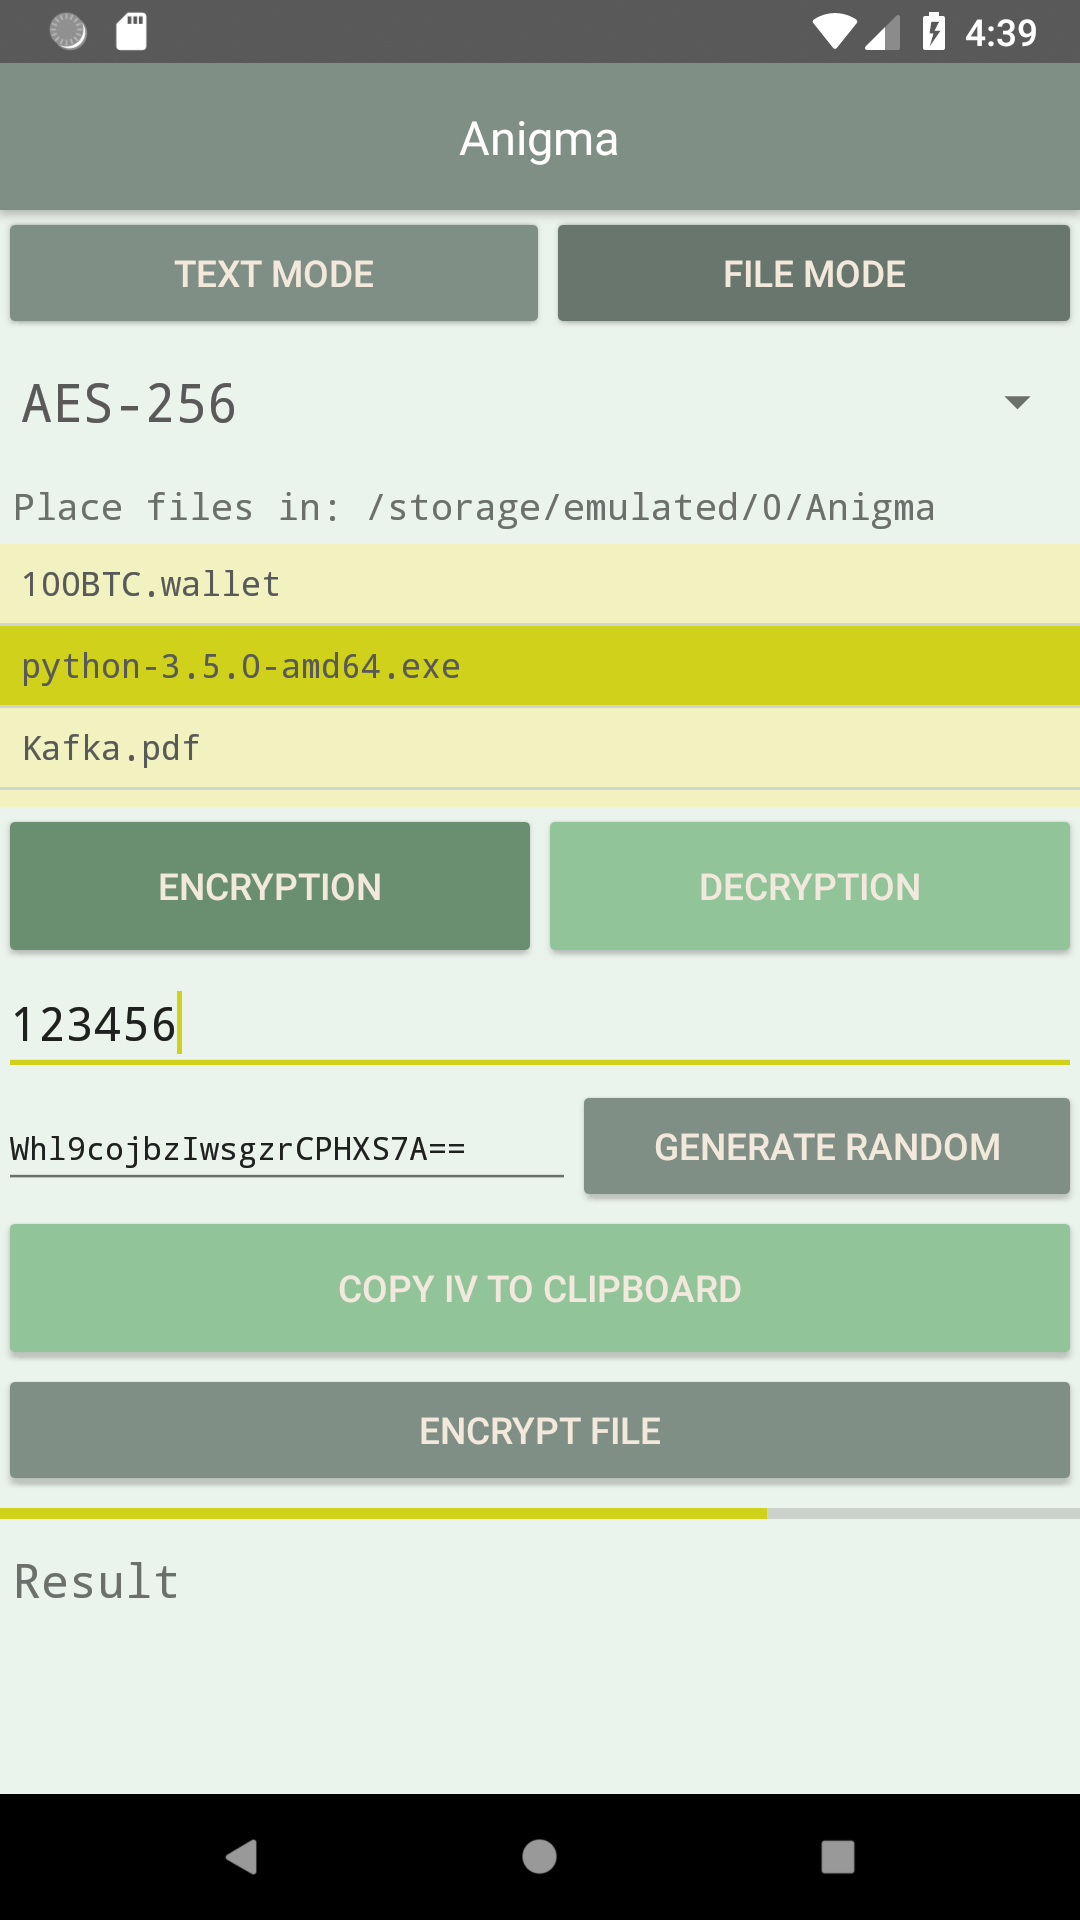
\includegraphics[height=0.4\textheight]{progress}
\label{fig:progress}
\end{figure}

\begin{figure}[h]
\caption{Zašifrovaný soubor.}
\centering
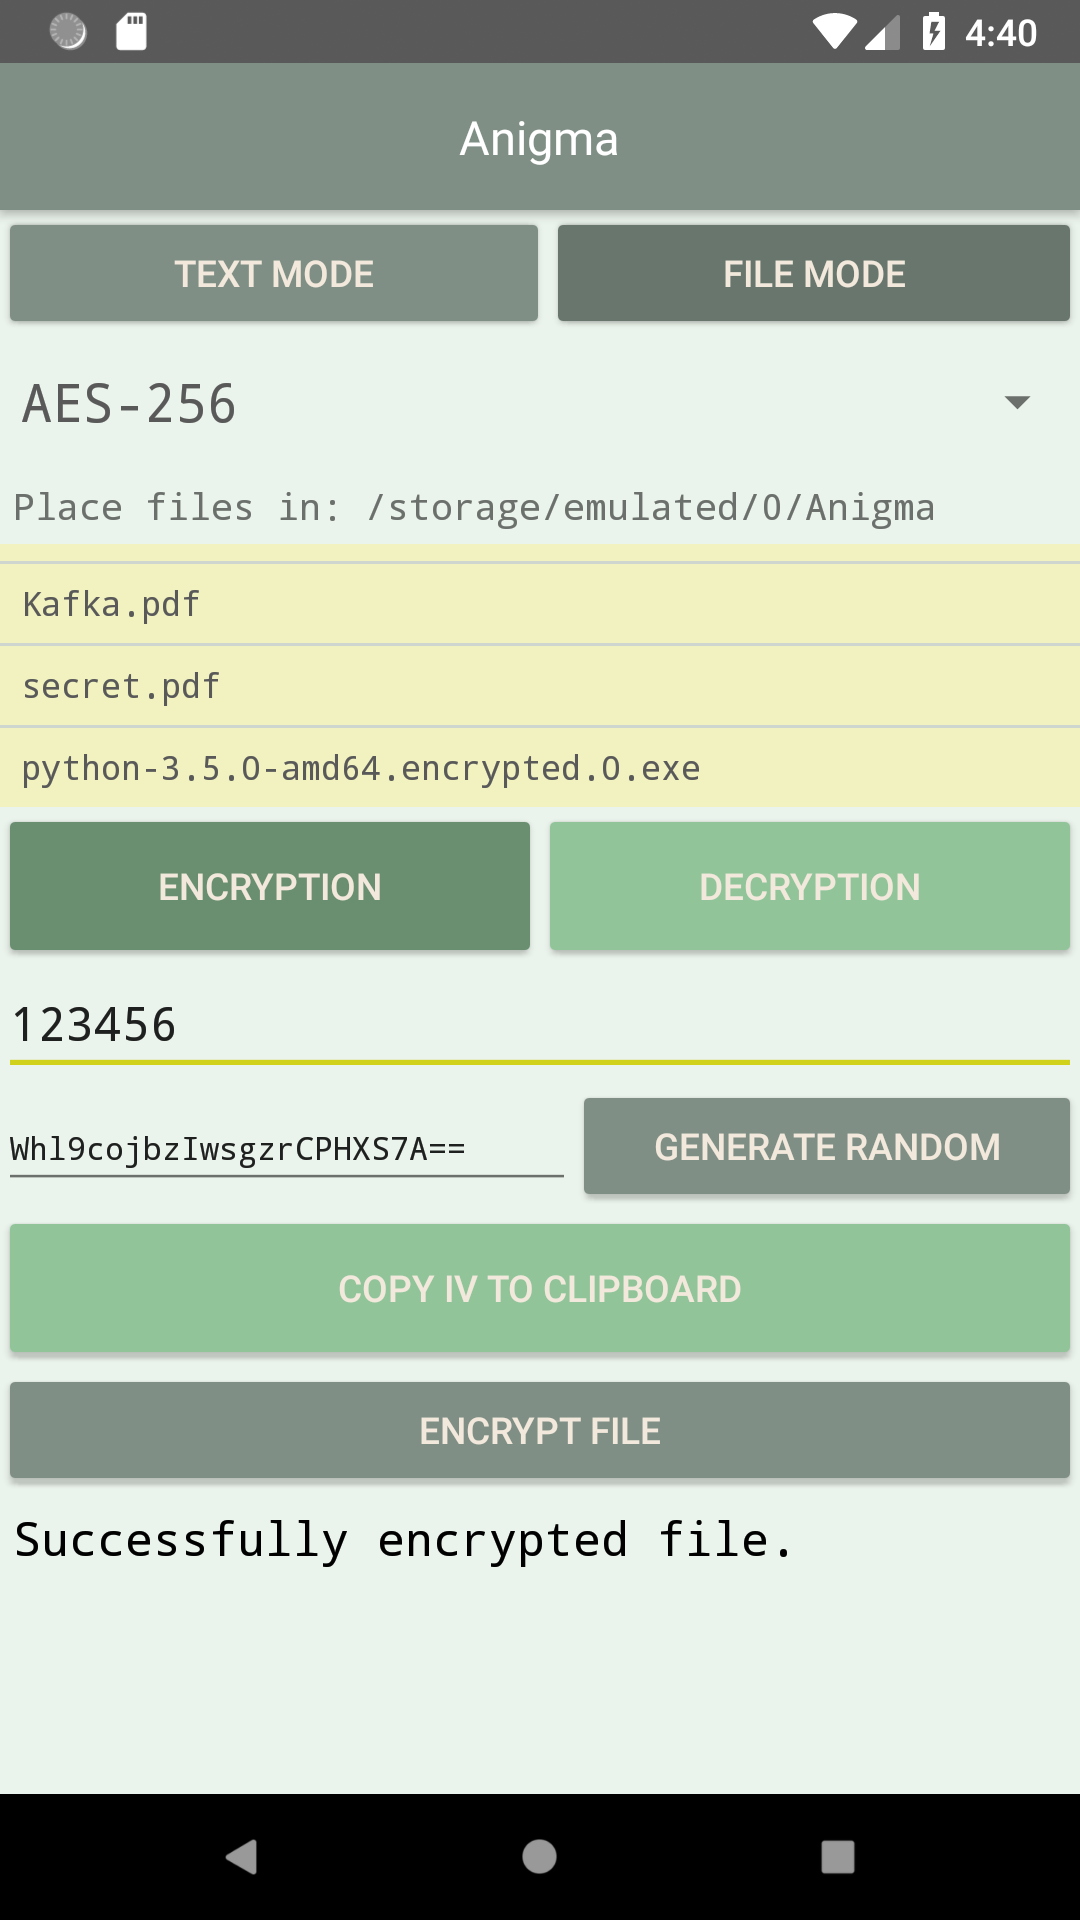
\includegraphics[height=0.4\textheight]{file_enc_success}
\label{fig:file_enc_success}
\end{figure}

\begin{figure}[h]
\caption{Dešifrovaný soubor.}
\centering
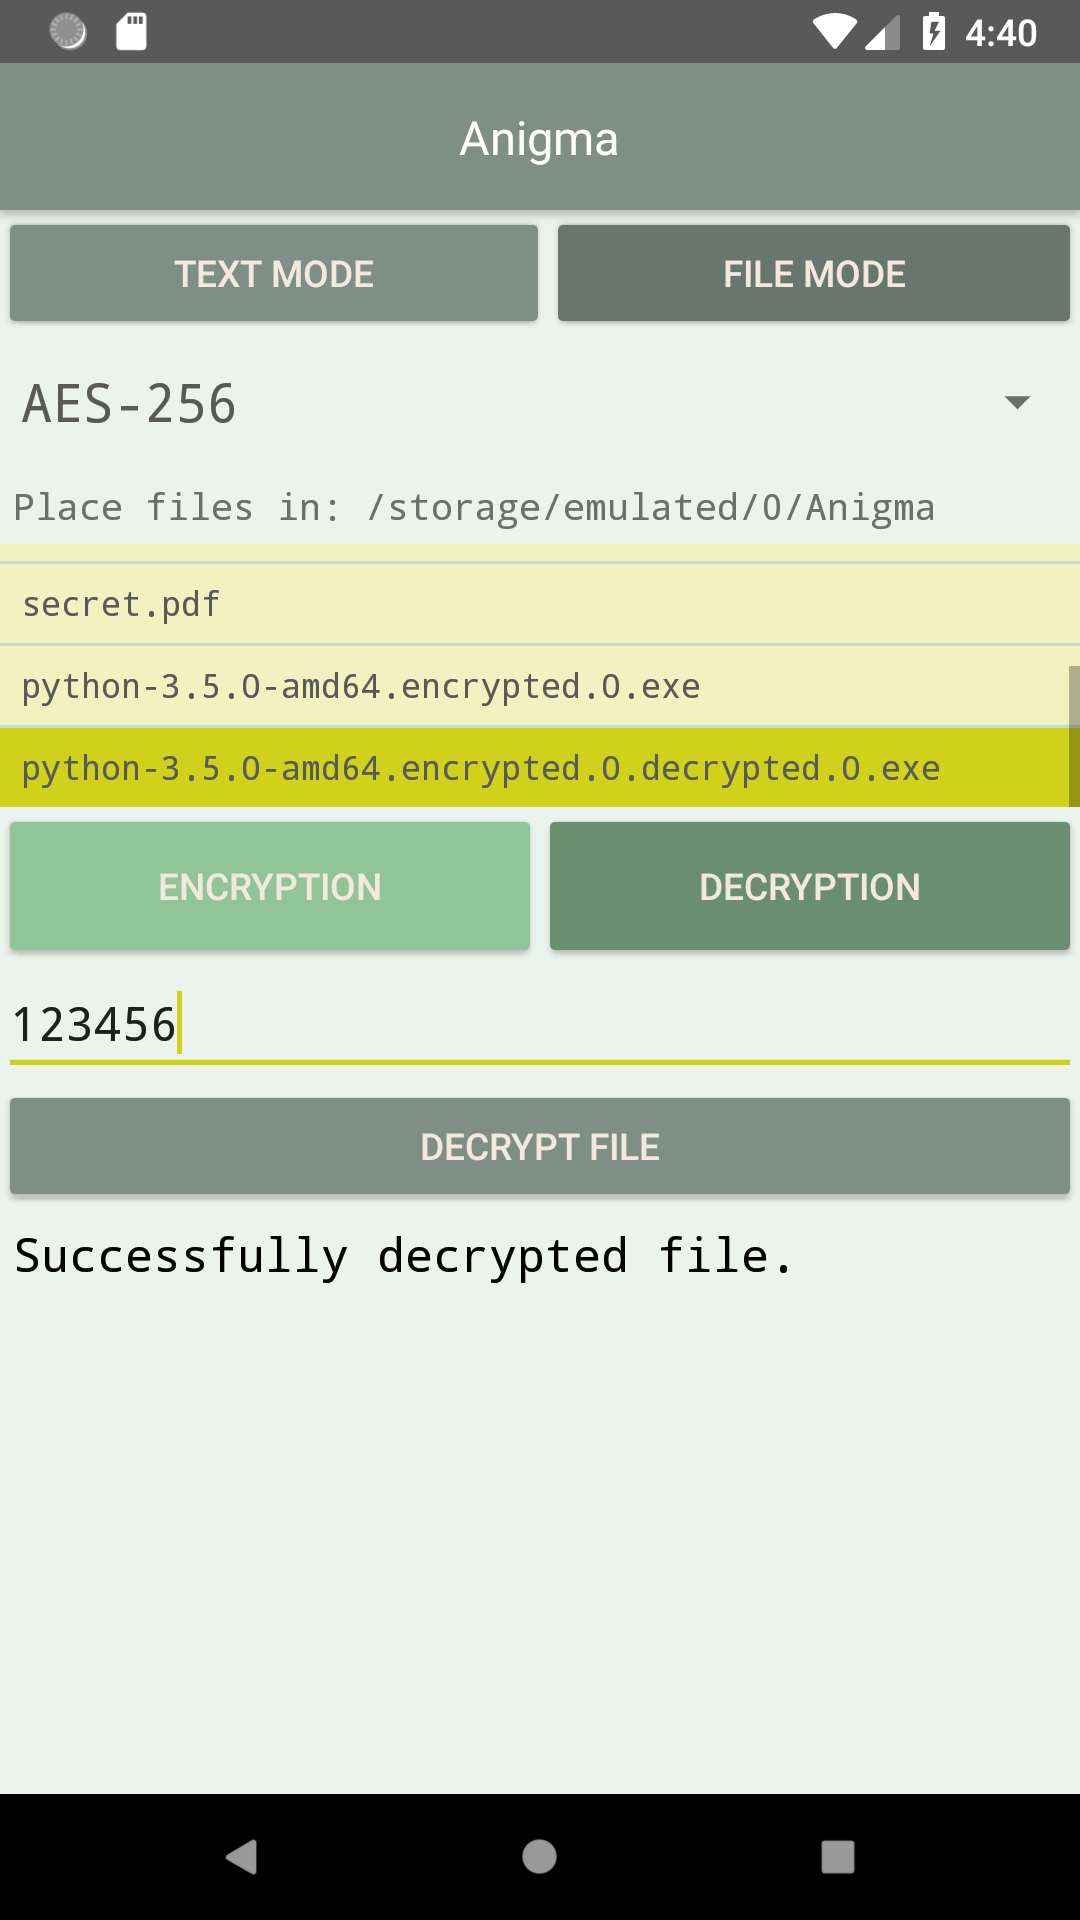
\includegraphics[height=0.4\textheight]{file_dec_success}
\label{fig:file_dec_success}
\end{figure}

\end{document}